\documentclass{article}
\usepackage[cm]{fullpage}
\usepackage{setspace}
\usepackage{amsmath}
\usepackage{booktabs}
\usepackage{dcolumn}
\usepackage{caption}
\usepackage{subcaption}

\title{STAT 209: Take-Home Problem Set 1}
\author{Rebecca Weiss}

\usepackage{Sweave}
\begin{document}
\Sconcordance{concordance:weiss_209_th1.tex:weiss_209_th1.Rnw:%
1 12 1 1 0 16 1 1 7 1 1 1 2 1 0 1 1 7 0 1 3 1 0 1 7 6 0 2 1 1 4 2 0 2 1 %
1 2 1 1 5 0 1 4 3 0 4 1 19 0 1 4 2 1 1 4 3 0 5 1 1 3 1 0 1 1 1 3 1 0 1 %
1 1 3 1 0 2 1 1 3 2 0 1 1 1 3 1 0 1 1 1 3 2 0 1 1 1 3 1 0 3 1 1 3 1 0 1 %
1 5 0 1 4 2 0 1 1 1 3 1 0 1 3 6 0 1 6 4 0 2 1 1 5 3 0 1 1 5 0 1 4 2 0 2 %
1 5 0 1 3 1 0 1 1 5 0 1 1 6 0 1 2 3 1 1 2 1 0 1 1 5 0 1 4 2 0 2 1 5 0 1 %
3 1 0 1 1 5 0 1 1 6 0 1 2 81 1 1 2 1 0 8 1 3 0 1 2 3 1 1 5 17 0 1 2 3 1 %
1 10 17 0 1 2 18 1 1 6 7 1 1 3 2 0 1 1 6 0 1 1 6 0 1 3 1 0 4 1 3 0 2 2 %
1 0 1 1 22 0 1 2 4 1 1 3 2 0 2 1 1 2 8 0 1 2 14 1 1 2 1 0 1 1 1 2 1 0 1 %
1 1 3 2 0 1 3 1 0 1 1 1 3 1 0 1 2 4 0 1 2 1 16 1 3 4 1 1 3 31 0 1 2 13 %
1}


\DefineVerbatimEnvironment{Sinput}{Verbatim} {xleftmargin=2em}
\DefineVerbatimEnvironment{Soutput}{Verbatim}{xleftmargin=2em}
\DefineVerbatimEnvironment{Scode}{Verbatim}{xleftmargin=2em}
\fvset{listparameters={\setlength{\topsep}{0pt}}}
\renewenvironment{Schunk}{\vspace{\topsep}}{\vspace{\topsep}}

\doublespacing

\maketitle



\section{Question 1: Observational studies, Associations}


\subsection{Part A: Spurious correlation}
\begin{Schunk}
\begin{Sinput}
> rm(list=ls(all=T))
> gc()
\end{Sinput}
\begin{Soutput}
         used (Mb) gc trigger (Mb) max used (Mb)
Ncells 198123 10.6     407500 21.8   350000 18.7
Vcells 317488  2.5     905753  7.0   863120  6.6
\end{Soutput}
\begin{Sinput}
> #Libraries
> library(mediation)
> #reconstruct the correlation matrix
> data = as.data.frame(cbind(
   c(1, -0.03, 0.39, -0.05, -0.08),
   c(-0.03, 1, 0.07, -0.23, -0.16),
   c(0.39, 0.07, 1, -0.13, -0.29),
 	c(-0.05, -0.23, -0.13, 1, 0.34),
 	c(-0.08, -0.16, -0.29, 0.34, 1)))
> rownames(data) = c('Exercise','Hardiness','Fitness','Stress','Illness')
> colnames(data) = c('Exercise','Hardiness','Fitness','Stress','Illness')
> #We need to see if the bivariate correlation of -0.27 changes compared to the partial correlation
> #let's look at the correlation between Fitness and Illness controlling for stress
> ryx = -0.29
> ryz = -0.13
> rxz = 0.34
> ryx.z = (ryx - (ryz*rxz)) / ( sqrt(1-(ryz^2)) * sqrt(1-(rxz^2)) )
> ryx.z
\end{Sinput}
\begin{Soutput}
[1] -0.263608
\end{Soutput}
\begin{Sinput}
> #this produces a partial correlation that is close to the zero order correlation between 
> #Fitness and Illness.  This implies that there is a direct effect, controlling for stress.
> #Here's an attempt at a significance test.  First, compute the partial correlation matrix:
> cor_mat = as.matrix(data)
> pcor_mat = solve(cor_mat) * -1
> diag(pcor_mat) = -diag(pcor_mat)
> pcor_mat = cov2cor(pcor_mat)
> cor.test(cor_mat, pcor_mat)
\end{Sinput}
\begin{Soutput}
	Pearson's product-moment correlation

data:  cor_mat and pcor_mat 
t = 45.6318, df = 23, p-value < 2.2e-16
alternative hypothesis: true correlation is not equal to 0 
95 percent confidence interval:
 0.9874112 0.9976215 
sample estimates:
      cor 
0.9945225 
\end{Soutput}
\begin{Sinput}
> #This shows that the correlation and partial correlation are not significantly different 
> #from each other at the 95% CI (because the correlation between these two matrices is nonzero)
\end{Sinput}
\end{Schunk}

\subsection{Part B: Stress as mediator}

\begin{Schunk}
\begin{Sinput}
> #STANDARDIZED METRICS
> #first, get the coef predictors for stress and fitness
> illness = c(-.08,-.16,-.29,.34)
> illness_pred_mat = data[1:4, 1:4]
> illness_coefs = solve(illness_pred_mat, illness)
> stress = c(-.05, -.23, -.13)
> stress_pred_mat = data[1:3, 1:3]
> stress_coefs = solve(stress_pred_mat, stress)
> #perform mediation analysis via sobel test
> names(illness_coefs) = names(data)[1:4] 
> names(stress_coefs) = names(data)[1:3]
> #get standard errors from correlation matrix
> illness_rsq = illness_coefs %*% illness
> stress_rsq = stress_coefs %*% stress
> #for illness
> n = 373
> illness_cov_beta = (1-illness_rsq)[1] * solve(illness_pred_mat)
> illness_serr = NA
> for (i in 1:length(diag(illness_cov_beta))){
 	illness_serr[i] = sqrt(as.numeric(diag(illness_cov_beta)[i])/n) * (n / (n-length(illness))) 
 }
> names(illness_serr) = names(illness_coefs)
> #for stress
> stress_cov_beta = (1-stress_rsq)[1] * solve(stress_pred_mat)
> stress_serr = NA
> for (i in 1:length(diag(stress_cov_beta))){
 	stress_serr[i] = sqrt(as.numeric(diag(stress_cov_beta)[i])/n) * (n / (n-length(illness)))
 }
> names(stress_serr) = names(stress_coefs)
> #here's some sloppy coding:
> illness_coefs = as.data.frame(t(illness_coefs))
> stress_coefs = as.data.frame(t(stress_coefs))
> illness_serr = as.data.frame(t(illness_serr))
> stress_serr = as.data.frame(t(stress_serr))
> #first step: indirect effect of stress on illness (mediating fitness and illness)
> indirect_effect = stress_coefs$Fitness * illness_coefs$Stress
> indirect_effect
\end{Sinput}
\begin{Soutput}
[1] -0.03166258
\end{Soutput}
\begin{Sinput}
> #get the effect variance and standard error
> effect_var = ((stress_coefs$Fitness)^2 * (illness_serr$Stress)^2) + 
   ( (illness_coefs$Stress)^2 * (stress_serr$Fitness)^2 )
> effect_serr = sqrt(effect_var)
> #finding the z value
> z = indirect_effect/effect_serr
> #do we just compare the z against the t distribution for significance?  are degrees of freedom n-1?
> print(pt(z, n-1))
\end{Sinput}
\begin{Soutput}
[1] 0.03090761
\end{Soutput}
\begin{Sinput}
> #UNSTANDARDIZED COEFFICIENTS
> #Unstandarized coefficient for y on x is the covariance of x and y over the variance of 
> #x.  Since we have all the standard deviations, we simply divide the coefficients by 
> #the variance of their corresponding X to get unstandardized coefficients.
> stdevs = c(66.50, 3.80, 18.40, 6.70, 624.80)
> vars = as.data.frame(t(stdevs^2))
> names(vars) = c('Exercise','Hardiness','Fitness','Stress','Illness')
> #now redo all of the previous steps, but with unstandardized coefficients
> 
> #first step: indirect effect of stress on illness (mediating fitness and illness)
> indirect_effect = (stress_coefs$Fitness / vars$Fitness) * (illness_coefs$Stress / vars$Stress)
> indirect_effect
\end{Sinput}
\begin{Soutput}
[1] -2.083344e-06
\end{Soutput}
\begin{Sinput}
> #get the effect variance and standard error
> effect_var = (((stress_coefs$Fitness)^2 / vars$Fitness) * ((illness_serr$Stress)^2 / vars$Stress) +
                 ((illness_coefs$Stress)^2 / vars$Stress) * ((stress_serr$Fitness)^2 / vars$Fitness))
>               effect_serr = sqrt(effect_var)
>               effect_serr
\end{Sinput}
\begin{Soutput}
[1] 0.0001371051
\end{Soutput}
\begin{Sinput}
>               #finding the z value
>               z = indirect_effect/effect_serr
>               z
\end{Sinput}
\begin{Soutput}
[1] -0.01519524
\end{Soutput}
\begin{Sinput}
>               pt(z, n-1)
\end{Sinput}
\begin{Soutput}
[1] 0.4939423
\end{Soutput}
\end{Schunk}
This is why we use standardized coefficients.  The z-score is nonsense.  This is because the original units that the variables were measured in are not compatible to each other.  This results in an insignificant finding.  

\subsection{Part C: Effects of errors in measurement}
Recall that reliability of a measure is the ratio of slopes.  Therefore, we can find the calculations by multiplying the slope coefficient by the reliability. If fitness has reliability 0.8 and stress has reliability 0.7, we can compute the following:
\begin{Schunk}
\begin{Sinput}
> indirect_effect = (stress_coefs$Fitness*0.8) * (illness_coefs$Stress*0.7)
> indirect_effect
\end{Sinput}
\begin{Soutput}
[1] -0.01773104
\end{Soutput}
\begin{Sinput}
> #get the effect variance and standard error
> effect_var = ((stress_coefs$Fitness * 0.8)^2 * (illness_serr$Stress)^2) + 
   ( (illness_coefs$Stress*0.7)^2 * (stress_serr$Fitness)^2 )
> effect_serr = sqrt(effect_var)
> effect_serr
\end{Sinput}
\begin{Soutput}
[1] 0.01201017
\end{Soutput}
\begin{Sinput}
>               #finding the z value
>               z = indirect_effect/effect_serr
>               z
\end{Sinput}
\begin{Soutput}
[1] -1.476335
\end{Soutput}
\begin{Sinput}
>               pt(z, n-1)
\end{Sinput}
\begin{Soutput}
[1] 0.07034993
\end{Soutput}
\end{Schunk}

And thus, the relationship is no longer significant.

\section{Question 2: Potential outcomes, Encouragement designs}

\subsection{Sodium intake on Systolic Blood Pressure}
For this question, we are evaluating an experiment that looked at whether sodium intake has some effect on cardiovascular health.  Since I don't know much at all about cardiology, I will assume that there was a theoretical reason to presume that a) systolic blood pressure is a useful indicator of cardiovascular health, particularly with respect to hypertension and b) there was a sound theoretical reason to hypothesize that sodium related to cardiovascular health (perhaps naive of me to assume that there are sound reasons behind hypotheses in medical research).

We are given tables 3 and 5.  The design of this study was as follows: participants were randomly assigned to either a treatment or control condition.  In treatment, participants were encouraged to reduce their sodium intake through an intervention program consisting  of counseling, dietary changes, group meetings, and so forth.  In control, participants were \emph{not encouraged} to make changes to their diet or lifestyle.  Systolic blood pressure and urinary sodium content were the measures of interest.

This is an encouragement design because of the very nature of treatment.  Much like Holland's example with students being encouraged to study more, and then evaluating the effect of amount of time studied on some outcome score, this experiment has two paths: the effect of assignment on the independent variable and the effect of the independent variable on the outcome variable.  Participants in treatment are encouraged to reduce their sodium intake, a treatment to which we assume must have varying degrees of success amongst assigned participants.  We note the average changes between the treatment and control conditions on sodium intake as well as systolic blood pressure, note significant differences via our favorite statistical inference test, and declare sodium intake to have a strong negative effect on cardiovascular health.

\subsubsection{Dose-response between systolic BP and sodium intake}

To estimate the unit-level effects, it is useful to revisit Holland's formulations.

First, with respect to treatment, we have assignment $S$ (or in Rogosa's slides, $G$), which results in the following variable $R(u, s)$:

\begin{quote}
$R(u, t)$ = amount $u$ decreases sodium intake if encouraged\\
$R(u, c)$ = amount $u$ decreases sodium intake if not encouraged
\end{quote}

Thus, outcome is not simply a function of $S$, but also of $R$, or more formally Y(u, s, r):

\begin{quote}
$Y(u, t, r)$ = systolic blood pressure for $u$ if $u$ is encouraged to decrease sodium intake and $u$ decreases sodium intake by $r$ amount\\
$Y(u, c, r)$ = systolic blood pressure for $u$ if $u$ is not encouraged to decrease sodium intake and $u$ decreases sodium intake by $r$ amount
\end{quote}

One important point to realize about encouragement designs is that not all combinations of R(u,s) and Y(u, s, r) are observable.  This results in a problem: we have no counterfactual data.  This is why a simple inferential test of sample means is problematic.  We must instead evaluate average causal effects over these variables, using notation from equations 24-27 from Holland: $\rho(u)$, $(r-r')\beta(u)$, $\tau(u)$, and the direct + indirect effect $\tau(u) + \rho(u)\beta(u)$.


\begin{figure}[!htf]
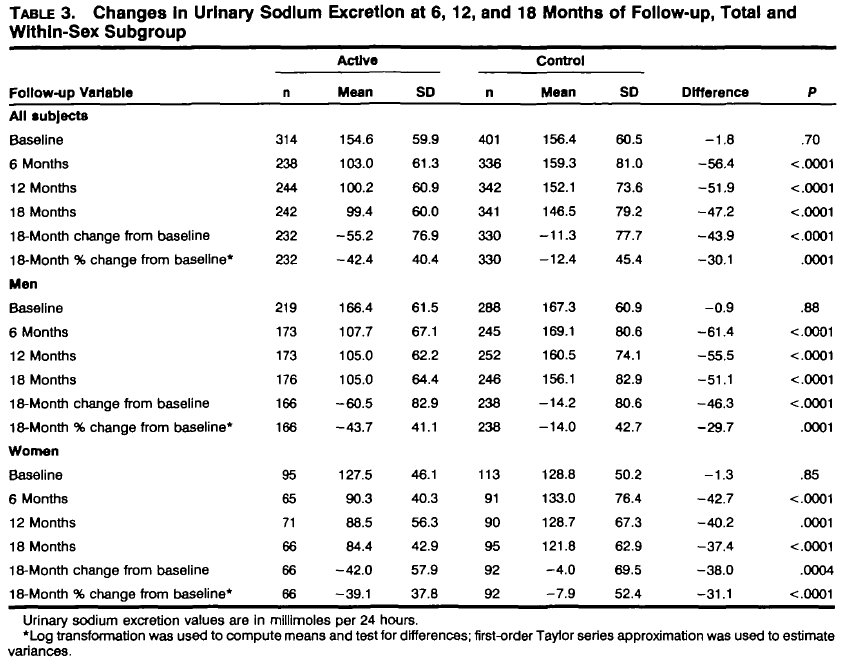
\includegraphics[width=\textwidth]{table3}
\end{figure}

\begin{figure}[!htf]
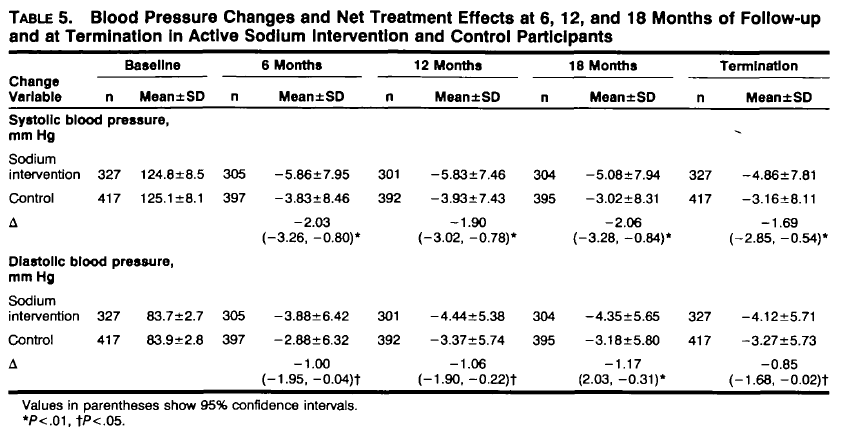
\includegraphics[width=\textwidth]{table5}
\end{figure}

\paragraph{Difference in amount of sodium intake for $u$ when in treatment vs. when in control (from table 3, from baseline between conditions)}
\begin{align*}
R_t(u) - R_c(u) &= \rho(u)\\
154.6 - 156.4 &= -1.80000000000001
\end{align*}

\paragraph{Difference in systolic blood pressure for reducing sodium intake by amount $r$ vs. reducing sodium intake by amount $r'$ (from table 5, 18 month change from baseline between conditions)}

\begin{align*}
Y_{Sr}(u) - Y_{Sr'}(u) = (r-r')\beta(u)\\
-5.08 + 3.02 = -2.06
\end{align*}

\paragraph{Difference in systolic blood pressure when in treatment vs. when in control with same amount of sodium intake $r$ (from table 5, baseline)}

\begin{align*}
Y_{tr}(u) - Y_{cr}(u) &= \tau(u) \\
124.8 - 125.1 &= -0.3
\end{align*}

\paragraph{Overall difference in systolic blood pressure score when in treatment vs. when in control}
\begin{align*}
Y_{tR_{t}}(u) - Y_{cR_{c}}(u) &= \tau(u) + \rho(u)\beta(u)\\
&= 3.40800000000003 
\end{align*}

\paragraph{Summary: } For every 3.10800000000003 decrease in salt intake, I estimate a unit decrease in systolic blood pressure.

\paragraph{What's the assumption underlying these estimators?}
We are assuming that \emph{individual differences} are not relevant between conditions.  In other words, we are assuming that there are no unobserved and influential covariates of participants that differ systematically between treatment versus control conditions, particularly those that interact with the treatment.  This presents a potential problem of bias.  For example, let's say the encouragement treatment is more effective at introducing novel lifestyle changes amongst young women more so than any other group.  Perhaps these unobserved lifestyle changes are also effective at lowering systolic blood pressure.  If these lifestyle changes are not observed and accounted for in this model, the effect of sodium intake on systolic blood pressure may be overestimated.  For the purposes of this study, it seems rather unlikely that certain subsamples of the sample would react that dramatically different to the intervention treatment, given its ultimate goal of reducing sodium intake.  

Additionally, we assume that the encouragement was the only factor leading to a difference in behavior between treatment and control.  This is because the implicit assumption is that control is acting as treatment would, had it not been for the treatment.  Because this is an \emph{encouragement}, it is difficult to be sure that 1) the treatment uniformally affect all those in the response-treatment condition and 2) those in the control didn't also spontaneously decide to make lifestyle changes.  Again, this is unusual and unlikely, given the nature of the behavior the authors were trying to change.

Holland alerts us to the importance of ALICE (additive, linear, causal effects).  This is a more formal explanation of this assumption: that the effects of the treatment are constant and don't depend on some intrinsic property of the unit (in this case, participants)

\subsection{Framing effects on Likelihood of Congressional Outreach}
In this study, Brader et al. (2008) presumed that exposure to certain kinds of media regarding immigration policy would induce a emotional response amongst exposed individuals, which would increase the probability that they would want to write their Congressman.  In this case, we have a treatment $S$ of \{Latino cue : European cue\}.  Our response variable is ``emo'', which is a 10pt measure of anxiety.  Our outcome variable is a binary treatment \{0 : 1\}, indicating whether a participant agreed to send a message to their Congressman or not.  

This resembles an encouragement design, albeit more subtly than the previous example.  Here, the encouragement is the frame; a Latino frame is ostensibly supposed to incur a different level of anxiety amongst participants as opposed to a European frame.  This effect, in line with much social science, is presumed to be an implicit effect, as it is a psychological construct.  Therefore, the measured variable ``emo'' is supposed to serve as an indicator as to whether the treatment elicited the appropriate response.  Additionally, the measured variable ``emo'' is presumed to be a mediator on ``cong\_mesg'', such that the probability that a person will submit a message to their Congressman is increased if anxiety is increased.

First, let's load the data and fit the models, \emph{lm} models ``model0'', ``model1'', and ``model2''.
\begin{Schunk}
\begin{Sinput}
> options(width=60)
> options(continue=" ")
> library(mediation)
> data(framing)
> attach(framing)
> model0 = lm(emo ~ treat)
> model1 = lm(cong_mesg ~ emo)
> model2 = lm(treat ~ cong_mesg)
> detach(framing)
\end{Sinput}
\end{Schunk}

\begin{table}[htb]
\begin{minipage}[b]{.5\linewidth}
\centering
\begin{tabular}{ c D{.}{.}{-1}D{.}{.}{-1}D{.}{.}{-1} } 
\hline 
  & \multicolumn{ 1 }{ c }{ Model 0 } & \multicolumn{ 1 }{ c }{ Model 1 } & \multicolumn{ 1 }{ c }{ Model 2 } \\ \hline
 %           & Model 0     & Model 1     & Model 2    \\ 
(Intercept) & 6.59 ^{***} & -0.11       & 0.23 ^{***}\\ 
            & (0.19)      & (0.07)      & (0.03)     \\ 
cong\_mesg &             &             & 0.09       \\ 
            &             &             & (0.06)     \\ 
treat       & 1.48 ^{***} &             &            \\ 
            & (0.38)      &             &            \\ 
emo         &             & 0.06 ^{***} &            \\ 
            &             & (0.01)      &             \\
 $N$         & 265         & 265         & 265        \\ 
$R^2$       & 0.05        & 0.14        & 0.01       \\ 
adj. $R^2$  & 0.05        & 0.13        & 0.01       \\ 
Resid. sd   & 2.70        & 0.44        & 0.44        \\ \hline
 \multicolumn{4}{l}{\footnotesize{Standard errors in parentheses}}\\
\multicolumn{4}{l}{\footnotesize{$^\dagger$ significant at $p<.10$; $^* p<.05$; $^{**} p<.01$; $^{***} p<.001$}} 
\end{tabular} \captionof{table}{Males and Females}
\end{minipage}%
\begin{minipage}[b]{.5\linewidth}
\centering
\begin{tabular}{ c D{.}{.}{-1}D{.}{.}{-1}D{.}{.}{-1} } 
\hline 
  & \multicolumn{ 1 }{ c }{ Model 0 } & \multicolumn{ 1 }{ c }{ Model 1 } & \multicolumn{ 1 }{ c }{ Model 2 } \\ \hline
 %           & Model 0     & Model 1     & Model 2    \\ 
(Intercept) & 6.76 ^{***} & -0.12       & 0.27 ^{***}\\ 
            & (0.27)      & (0.10)      & (0.04)     \\ 
cong\_mesg &             &             & 0.01       \\ 
            &             &             & (0.08)     \\ 
treat       & 1.16 ^*     &             &            \\ 
            & (0.52)      &             &            \\ 
emo         &             & 0.06 ^{***} &            \\ 
            &             & (0.01)      &             \\
 $N$         & 139         & 139         & 139        \\ 
$R^2$       & 0.04        & 0.12        & 0.00       \\ 
adj. $R^2$  & 0.03        & 0.11        & -0.01      \\ 
Resid. sd   & 2.72        & 0.43        & 0.45        \\ \hline
 \multicolumn{4}{l}{\footnotesize{Standard errors in parentheses}}\\
\multicolumn{4}{l}{\footnotesize{$^\dagger$ significant at $p<.10$; $^* p<.05$; $^{**} p<.01$; $^{***} p<.001$}} 
\end{tabular} \captionof{table}{Females only}
\end{minipage}
\end{table}

\paragraph{What are the significant effects?}

\subparagraph{Treatment on ``emo'': }  According to the OLS model, the treatment does have a positive and significant effect on anxiety.  Being in the treatment condition increases anxiety by 1.48 units.  For females, this effect is smaller and less significant, 1.16 units.
\subparagraph{Treatment on ``cong\_mesg'': } According to the OLS model, anxiety does have a positive and significant effect on the probability that someone will send a message to their Congressman.  For every unit increase in anxiety, the probability of sending a message increases by 6\%.  For females, this effect is the same.
\subparagraph{Effect of unit changes in ``emo'' on probability of sending message to Congressmen: } Upon reviewing model 2, we see that the slope is $0.09$ and the intercept is $0.23$.   The slope is the change in outcome as treatment moves from 0 to 1.  The intercept is the baseline probability.  Interpreting these results according to those terms means that the baseline probability that someone will send a message to their Congressman, regardless of treatment or anxiety, is 23\%.  For females, the baseline is higher, 29\%.  

\paragraph{Can we make the same assumptions with this encouragement design as with the sodium intake example in 2a?}
No.  There are several indicators that individual differences interact with the response to the treatment.  First, there are baseline differences between males and females regarding their probability of sending a message to a Congressman regardless of their treatment.  Second, the effect of the treatment on anxiety is different.  Women do not react as strongly to the treatment with respect to elevated levels of anxiety, and yet the effect of anxiety on probability of sending a message to a Congressman is the same between males and females.

Consider, also, that there it's not clear that those in the control condition should be considered identical to those in the treatment condition, aside from the framing encouragement.  Perhaps there were additional unobserved events that occurred 

ALICE

\section{Question 3: Multilevel Data, Random effects models}


\subsection{Compute the traditional quantities for ``normexam'' predicted by prior test score ``standLRT''}

There are two models that we can use to try to explore the relationship that this metric ``standLRT'' has with ``normexam.''  One is a simple OLS, regressing the school average score ``schavg'' on the outcome variable ``normexam.''  This model essentialy assumes that there are no significant differences between students at various schools.  A better model would be to try and account for the fixed effect of student variance within schools.

\paragraph{Part A: Aggregation bias} 
First, let's evaluate this relationship at the school level, using school-level means. 

\begin{Schunk}
\begin{Sinput}
> #is the distribution of the schavg is the same as the actual within school mean standLRT 
> options(width=60)
> summary(unique(schavg))
\end{Sinput}
\begin{Soutput}
    Min.  1st Qu.   Median     Mean  3rd Qu.     Max. 
-0.75600 -0.24170 -0.04053 -0.03075  0.21030  0.63770 
\end{Soutput}
\begin{Sinput}
> summary(tapply(standLRT, school, mean))
\end{Sinput}
\begin{Soutput}
    Min.  1st Qu.   Median     Mean  3rd Qu.     Max. 
-0.75600 -0.24170 -0.04053 -0.03075  0.21030  0.63770 
\end{Soutput}
\begin{Sinput}
> #Also, school 48 seems to be really throwing off the boxplot, so I'm going to get rid of it for now
> meannormexam = tapply(Exam$normexam, Exam$school, mean)
> Exam$meannormexam = meannormexam[Exam$school]
> Exam = Exam[!Exam$school %in% 48,]
> Exam_school = Exam[!duplicated(Exam[,'school']),]
> model_agg = lm(meannormexam ~ schavg, data=Exam_school)
\end{Sinput}
\end{Schunk}

\begin{Schunk}
\begin{Sinput}
> options(width=60)
> summary(model_agg)
\end{Sinput}
\begin{Soutput}
Call:
lm(formula = meannormexam ~ schavg, data = Exam_school)

Residuals:
     Min       1Q   Median       3Q      Max 
-1.15701 -0.14005 -0.00513  0.19993  0.66298 

Coefficients:
            Estimate Std. Error t value Pr(>|t|)    
(Intercept) 0.005325   0.040302   0.132    0.895    
schavg      0.880943   0.118093   7.460 3.43e-10 ***
---
Signif. codes:  0 ‘***’ 0.001 ‘**’ 0.01 ‘*’ 0.05 ‘.’ 0.1 ‘ ’ 1 

Residual standard error: 0.3216 on 62 degrees of freedom
Multiple R-squared: 0.473,	Adjusted R-squared: 0.4645 
F-statistic: 55.65 on 1 and 62 DF,  p-value: 3.43e-10 
\end{Soutput}
\end{Schunk}

According to the aggregated model, for every unit increase in ``schavg,'' normexam will increase by 0.881.  The intercept is 0.00532. Thus, we might be tempted to say that the way to improve the normalized exam score is simply to accept the students with the highest entering scores. This is hardly compelling policy and begs the question: are all students within schools essentially identical?  

\paragraph{Part B: Contextual effects }  What is the (supposed) estimate of the effect on ``normexam'' for a student being in a school with one unit higher mean score on ``standLRT'' and student ``held constant?''.  This is akin to asking, what is the average slope and intercept over all individual regressions ``normexam'' on ``cstandLRT'' fit for each school.  As opposed to the aggregated model, the estimates for the slope and intercept are slightly different.  

\begin{Schunk}
\begin{Sinput}
> #Centering within-school individual scores using school means
> library(lme4)
> Exam$cstandLRT = Exam$standLRT - Exam$schavg
> model_lmlist = lmList(normexam ~ cstandLRT|school, Exam)
> #fixed effects are the same as taking the mean Intercept and Slopes for the centered standLRT metric
> sapply(coef(model_lmlist), mean)
\end{Sinput}
\begin{Soutput}
(Intercept)   cstandLRT 
-0.01648814  0.53905282 
\end{Soutput}
\end{Schunk}

According to this model, the true effect on normexam is 0.539, with the intercept at -0.0165.  This is a rather large difference in slope than the aggregated model, which indicates an \emph{aggregation bias} of  0.342.

\subsection{Gender differences in outcome (the ``gender gap'') for the coed (``mixed'') schools}

\paragraph{\textbf{Part C: } Give a point estimate and standard error for gender differences in outcome for these multilevel data}

First, let's formally define the models that we are looking at.  We're interested 

At another level, we recognize that each individual school might operate slightly differently, and that using a mean measure of a school actually results in a loss of information about the statistical relationships between the variables of interest.  Level 1 is the within-schools regression, looking at each individual $j$ in school $i$.  Level 2 is over all schools, acknowledging the effect of average standLRT performance and gender.

\subparagraph{Level 1: } $normexam$ = $\alpha_{0i}$ + $\alpha_{1i}cstandLRT_{ij}$ + $\epsilon_{ij}$
\subparagraph{Level 2: $\alpha_{0i}$}=  $\gamma_{00}$ + $\gamma_{01}schavg$ + $\gamma_{02}sex_{i}$ + $u_{0i}$
\subparagraph{Level 2: $\alpha_{1i}$}=  $\gamma_{10}$ + $\gamma_{11}schavg$ + $\gamma_{12}sex_{i}$ + $u_{1i}$

\begin{Schunk}
\begin{Sinput}
> options(width=60)
> options(continue=" ")
> #First, subset down to only mixed-gender schools
> Exam_mxd = Exam[Exam$type == 'Mxd',]
> Exam_mxd$sex = factor(Exam_mxd$sex, levels=c('M','F'))
> #FYI, schools 43 and 47 barely count as coed, should drop them
> #table(sex, school)
> Exam_mxd = Exam_mxd[!Exam_mxd$school %in% c(43, 47),]
> #using lmList
> model_lvl1_XX = lmList(normexam ~ cstandLRT|school, subset = sex == 'F', data=Exam_mxd)
> model_lvl1_XY = lmList(normexam ~ cstandLRT|school, subset = sex == 'M', data=Exam_mxd)
> #using lmer
> library(lme4)
> model_lvl2_lmer = lme4::lmer(normexam ~ schavg*cstandLRT + sex*cstandLRT + 
                                (1 + cstandLRT|school), data = Exam_mxd)
\end{Sinput}
\end{Schunk}

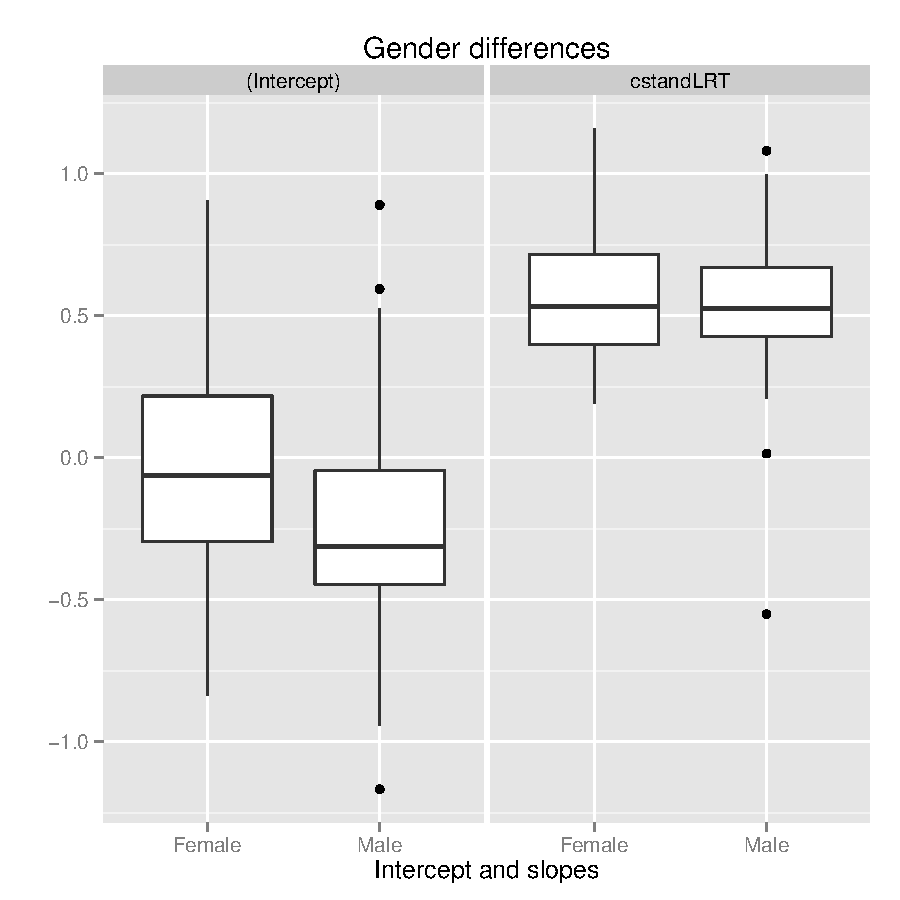
\includegraphics{weiss_209_th1-3cd_plot}

As you can see from the graph, there is a gender effect on the intercept.  The boxplot indicates that females have somewhat stronger performance within the schools on average, and the slopes on cstandLRT are relatively the same.  

This is supported by the output below:

\begin{Schunk}
\begin{Soutput}
Linear mixed model fit by REML 
Formula: normexam ~ schavg * cstandLRT + sex * cstandLRT + (1 + cstandLRT |      school) 
   Data: Exam_mxd 
  AIC  BIC logLik deviance REMLdev
 4591 4647  -2286     4547    4571
Random effects:
 Groups   Name        Variance  Std.Dev. Corr  
 school   (Intercept) 0.0922683 0.303757       
          cstandLRT   0.0074176 0.086125 0.509 
 Residual             0.5292113 0.727469       
Number of obs: 2026, groups: school, 33

Fixed effects:
                  Estimate Std. Error t value
(Intercept)      -0.159155   0.058561  -2.718
schavg            0.934706   0.177825   5.256
cstandLRT         0.556726   0.028296  19.675
sexF              0.169522   0.033376   5.079
schavg:cstandLRT  0.133952   0.077442   1.730
cstandLRT:sexF    0.008816   0.035436   0.249

Correlation of Fixed Effects:
            (Intr) schavg cstLRT sexF   sc:LRT
schavg       0.105                            
cstandLRT    0.276  0.029                     
sexF        -0.276 -0.004 -0.048              
schvg:csLRT  0.033  0.298  0.149  0.002       
cstndLRT:sF -0.021  0.002 -0.534 -0.003  0.007
\end{Soutput}
\end{Schunk}


\paragraph{\textbf{Part D:} Do these gender differences have any association with ``intake''}

\begin{itemize}
  \item This model is pegged against males as the baseline.  The fixed-effect of -0.159 is the average level of performance on normexam of males.  
  \item The coefficient for sexF is 0.17 and it represents the average performance of females on the normexam relative to males.  In other words, females are performing better than males, on average, within schools.
  \item The coefficient for schavg is 0.935, which is a school's average normexam performance to their average standLRT scores.  in other words, for each unit increase in schavg, normexam will increase by 0.935 on average.
  \item The coefficient for cstandLRT is the average slope for standLRT for all males in these schools.  Contrast that with the coefficient for cstandLRT:sexF, which is the average slope for all females.  The slope is smaller, on average, for females.
  \item The coefficient for schavg:cstandLRT is 0.134, which represents the average change in the within-school cstandLRT slope given a one-increment increase in the school average.  In other words, if a school's average (schavg) were to increase by one unit, the slope for that school's cstandLRT would increase by 0.935.
\end{itemize}


\end{document}
